\chapter{Cây khung}

\index{spanning tree}
\index{cây khung}

Một \key{cây khung} của một đồ thị bao gồm
tất cả các đỉnh của đồ thị và một số
cạnh của đồ thị sao cho có một đường đi
giữa hai đỉnh bất kỳ.
Giống như cây nói chung, cây khung
liên thông và không có chu trình.
Thông thường có một vài cách để xây dựng một cây khung.

Ví dụ, xét đồ thị sau:
\begin{center}
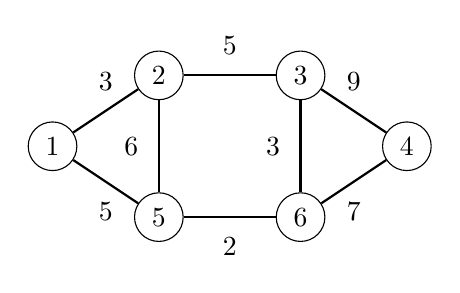
\begin{tikzpicture}[scale=0.9]
\node[draw, circle] (1) at (1.5,2) {$1$};
\node[draw, circle] (2) at (3,3) {$2$};
\node[draw, circle] (3) at (5,3) {$3$};
\node[draw, circle] (4) at (6.5,2) {$4$};
\node[draw, circle] (5) at (3,1) {$5$};
\node[draw, circle] (6) at (5,1) {$6$};
\path[draw,thick,-] (1) -- node[font=\small,label=above:3] {} (2);
\path[draw,thick,-] (2) -- node[font=\small,label=above:5] {} (3);
\path[draw,thick,-] (3) -- node[font=\small,label=above:9] {} (4);
\path[draw,thick,-] (1) -- node[font=\small,label=below:5] {} (5);
\path[draw,thick,-] (5) -- node[font=\small,label=below:2] {} (6);
\path[draw,thick,-] (6) -- node[font=\small,label=below:7] {} (4);
\path[draw,thick,-] (2) -- node[font=\small,label=left:6] {} (5);
\path[draw,thick,-] (3) -- node[font=\small,label=left:3] {} (6);
\end{tikzpicture}
\end{center}
Một cây khung cho đồ thị như sau:
\begin{center}
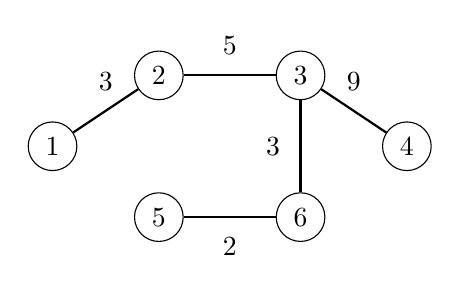
\begin{tikzpicture}[scale=0.9]
\node[draw, circle] (1) at (1.5,2) {$1$};
\node[draw, circle] (2) at (3,3) {$2$};
\node[draw, circle] (3) at (5,3) {$3$};
\node[draw, circle] (4) at (6.5,2) {$4$};
\node[draw, circle] (5) at (3,1) {$5$};
\node[draw, circle] (6) at (5,1) {$6$};
\path[draw,thick,-] (1) -- node[font=\small,label=above:3] {} (2);
\path[draw,thick,-] (2) -- node[font=\small,label=above:5] {} (3);
\path[draw,thick,-] (3) -- node[font=\small,label=above:9] {} (4);
\path[draw,thick,-] (5) -- node[font=\small,label=below:2] {} (6);
\path[draw,thick,-] (3) -- node[font=\small,label=left:3] {} (6);
\end{tikzpicture}
\end{center}

Trọng số của một cây khung là tổng trọng số các cạnh của nó.
Ví dụ, trọng số của cây khung trên là
$3+5+9+3+2=22$.

\index{minimum spanning tree}
\index{cây khung nhỏ nhất}

Một \key{cây khung nhỏ nhất}
là một cây khung có trọng số nhỏ nhất có thể.
Trọng số của một cây khung nhỏ nhất cho đồ thị ví dụ
là 20, và một cây như vậy có thể được xây dựng như sau:

\begin{center}
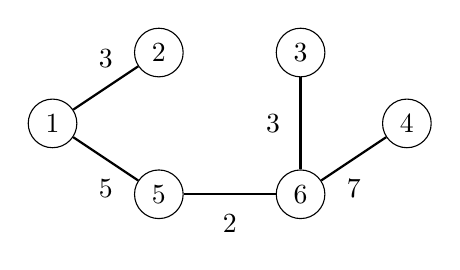
\begin{tikzpicture}[scale=0.9]
\node[draw, circle] (1) at (1.5,2) {$1$};
\node[draw, circle] (2) at (3,3) {$2$};
\node[draw, circle] (3) at (5,3) {$3$};
\node[draw, circle] (4) at (6.5,2) {$4$};
\node[draw, circle] (5) at (3,1) {$5$};
\node[draw, circle] (6) at (5,1) {$6$};

\path[draw,thick,-] (1) -- node[font=\small,label=above:3] {} (2);
\path[draw,thick,-] (1) -- node[font=\small,label=below:5] {} (5);
\path[draw,thick,-] (5) -- node[font=\small,label=below:2] {} (6);
\path[draw,thick,-] (6) -- node[font=\small,label=below:7] {} (4);
\path[draw,thick,-] (3) -- node[font=\small,label=left:3] {} (6);
\end{tikzpicture}
\end{center}

\index{maximum spanning tree}
\index{cây khung lớn nhất}

Tương tự, một \key{cây khung lớn nhất}
là một cây khung có trọng số lớn nhất có thể.
Trọng số của một cây khung lớn nhất cho
đồ thị ví dụ là 32:

\begin{center}
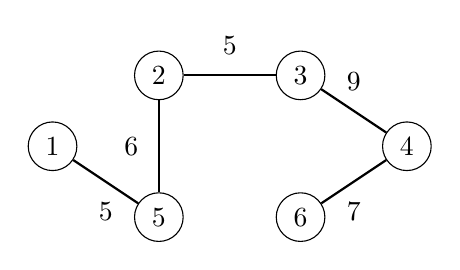
\begin{tikzpicture}[scale=0.9]
\node[draw, circle] (1) at (1.5,2) {$1$};
\node[draw, circle] (2) at (3,3) {$2$};
\node[draw, circle] (3) at (5,3) {$3$};
\node[draw, circle] (4) at (6.5,2) {$4$};
\node[draw, circle] (5) at (3,1) {$5$};
\node[draw, circle] (6) at (5,1) {$6$};
\path[draw,thick,-] (2) -- node[font=\small,label=above:5] {} (3);
\path[draw,thick,-] (3) -- node[font=\small,label=above:9] {} (4);
\path[draw,thick,-] (1) -- node[font=\small,label=below:5] {} (5);
\path[draw,thick,-] (6) -- node[font=\small,label=below:7] {} (4);
\path[draw,thick,-] (2) -- node[font=\small,label=left:6] {} (5);
\end{tikzpicture}
\end{center}

Lưu ý rằng một đồ thị có thể có một vài
cây khung nhỏ nhất và lớn nhất,
vì vậy các cây không phải là duy nhất.

Hóa ra một số phương pháp tham lam
có thể được sử dụng để xây dựng cây khung nhỏ nhất và lớn nhất.
Trong chương này, chúng ta thảo luận về hai thuật toán
xử lý các cạnh của đồ thị được sắp xếp theo trọng số của chúng.
Chúng ta tập trung vào việc tìm cây khung nhỏ nhất,
nhưng các thuật toán tương tự có thể tìm
cây khung lớn nhất bằng cách xử lý các cạnh theo thứ tự ngược lại.

\section{Thuật toán Kruskal}

\index{Kruskal's algorithm}
\index{thuật toán Kruskal}

Trong \key{thuật toán Kruskal}\footnote{Thuật toán được công bố năm 1956
bởi J. B. Kruskal \cite{kru56}.}, cây khung ban đầu
chỉ chứa các đỉnh của đồ thị
và không chứa bất kỳ cạnh nào.
Sau đó, thuật toán duyệt qua các cạnh
theo thứ tự trọng số của chúng, và luôn thêm một cạnh
vào cây nếu nó không tạo ra một chu trình.

Thuật toán duy trì các thành phần
của cây.
Ban đầu, mỗi đỉnh của đồ thị
thuộc về một thành phần riêng biệt.
Luôn luôn khi một cạnh được thêm vào cây,
hai thành phần được hợp nhất.
Cuối cùng, tất cả các đỉnh thuộc về cùng một thành phần,
và một cây khung nhỏ nhất đã được tìm thấy.

\subsubsection{Ví dụ}

\begin{samepage}
Hãy xem xét cách thuật toán Kruskal xử lý
đồ thị sau:
\begin{center}
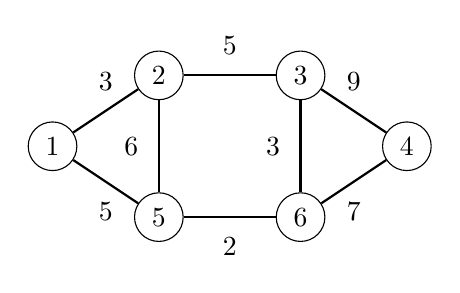
\begin{tikzpicture}[scale=0.9]
\node[draw, circle] (1) at (1.5,2) {$1$};
\node[draw, circle] (2) at (3,3) {$2$};
\node[draw, circle] (3) at (5,3) {$3$};
\node[draw, circle] (4) at (6.5,2) {$4$};
\node[draw, circle] (5) at (3,1) {$5$};
\node[draw, circle] (6) at (5,1) {$6$};
\path[draw,thick,-] (1) -- node[font=\small,label=above:3] {} (2);
\path[draw,thick,-] (2) -- node[font=\small,label=above:5] {} (3);
\path[draw,thick,-] (3) -- node[font=\small,label=above:9] {} (4);
\path[draw,thick,-] (1) -- node[font=\small,label=below:5] {} (5);
\path[draw,thick,-] (5) -- node[font=\small,label=below:2] {} (6);
\path[draw,thick,-] (6) -- node[font=\small,label=below:7] {} (4);
\path[draw,thick,-] (2) -- node[font=\small,label=left:6] {} (5);
\path[draw,thick,-] (3) -- node[font=\small,label=left:3] {} (6);
\end{tikzpicture}
\end{center}
\end{samepage}

\begin{samepage}
Bước đầu tiên của thuật toán là sắp xếp các
cạnh theo thứ tự tăng dần của trọng số của chúng.
Kết quả là danh sách sau:

\begin{tabular}{ll}
\\
cạnh & trọng số \\
\hline
5--6 & 2 \\
1--2 & 3 \\
3--6 & 3 \\
1--5 & 5 \\
2--3 & 5 \\
2--5 & 6 \\
4--6 & 7 \\
3--4 & 9 \\
\\
\end{tabular}
\end{samepage}

Sau đó, thuật toán duyệt qua danh sách
và thêm mỗi cạnh vào cây nếu nó nối
hai thành phần riêng biệt.

Ban đầu, mỗi đỉnh nằm trong thành phần riêng của nó:

\begin{center}
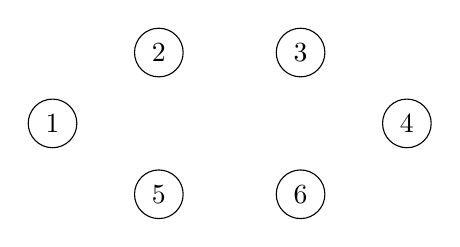
\begin{tikzpicture}[scale=0.9]
\node[draw, circle] (1) at (1.5,2) {$1$};
\node[draw, circle] (2) at (3,3) {$2$};
\node[draw, circle] (3) at (5,3) {$3$};
\node[draw, circle] (4) at (6.5,2) {$4$};
\node[draw, circle] (5) at (3,1) {$5$};
\node[draw, circle] (6) at (5,1) {$6$};
%\path[draw,thick,-] (1) -- node[font=\small,label=above:3] {} (2);
%\path[draw,thick,-] (2) -- node[font=\small,label=above:5] {} (3);
%\path[draw,thick,-] (3) -- node[font=\small,label=above:9] {} (4);
%\path[draw,thick,-] (1) -- node[font=\small,label=below:5] {} (5);
%\path[draw,thick,-] (5) -- node[font=\small,label=below:2] {} (6);
%\path[draw,thick,-] (6) -- node[font=\small,label=below:7] {} (4);
%\path[draw,thick,-] (2) -- node[font=\small,label=left:6] {} (5);
%\path[draw,thick,-] (3) -- node[font=\small,label=left:3] {} (6);
\end{tikzpicture}
\end{center}
Cạnh đầu tiên được thêm vào cây là
cạnh 5--6 tạo ra một thành phần $\{5,6\}$
bằng cách nối các thành phần $\{5\}$ và $\{6\}$:

\begin{center}
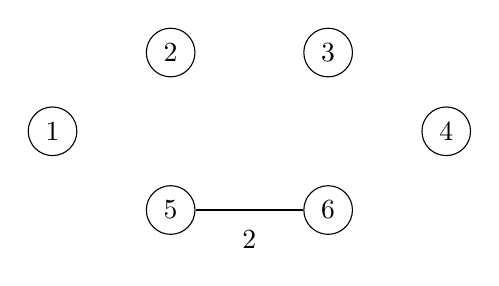
\begin{tikzpicture}
\node[draw, circle] (1) at (1.5,2) {$1$};
\node[draw, circle] (2) at (3,3) {$2$};
\node[draw, circle] (3) at (5,3) {$3$};
\node[draw, circle] (4) at (6.5,2) {$4$};
\node[draw, circle] (5) at (3,1) {$5$};
\node[draw, circle] (6) at (5,1) {$6$};

%\path[draw,thick,-] (1) -- node[font=\small,label=above:3] {} (2);
%\path[draw,thick,-] (2) -- node[font=\small,label=above:5] {} (3);
%\path[draw,thick,-] (3) -- node[font=\small,label=above:9] {} (4);
%\path[draw,thick,-] (1) -- node[font=\small,label=below:5] {} (5);
\path[draw,thick,-] (5) -- node[font=\small,label=below:2] {} (6);
%\path[draw,thick,-] (6) -- node[font=\small,label=below:7] {} (4);
%\path[draw,thick,-] (2) -- node[font=\small,label=left:6] {} (5);
%\path[draw,thick,-] (3) -- node[font=\small,label=left:3] {} (6);
\end{tikzpicture}
\end{center}
Sau đó, các cạnh 1--2, 3--6 và 1--5 được thêm vào một cách tương tự:

\begin{center}
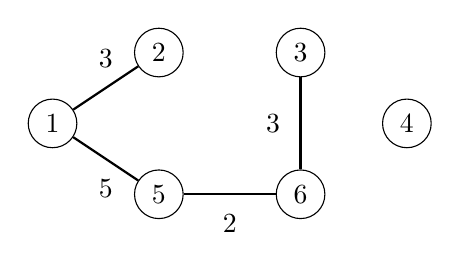
\begin{tikzpicture}[scale=0.9]
\node[draw, circle] (1) at (1.5,2) {$1$};
\node[draw, circle] (2) at (3,3) {$2$};
\node[draw, circle] (3) at (5,3) {$3$};
\node[draw, circle] (4) at (6.5,2) {$4$};
\node[draw, circle] (5) at (3,1) {$5$};
\node[draw, circle] (6) at (5,1) {$6$};

\path[draw,thick,-] (1) -- node[font=\small,label=above:3] {} (2);
%\path[draw,thick,-] (2) -- node[font=\small,label=above:5] {} (3);
%\path[draw,thick,-] (3) -- node[font=\small,label=above:9] {} (4);
\path[draw,thick,-] (1) -- node[font=\small,label=below:5] {} (5);
\path[draw,thick,-] (5) -- node[font=\small,label=below:2] {} (6);
%\path[draw,thick,-] (6) -- node[font=\small,label=below:7] {} (4);
%\path[draw,thick,-] (2) -- node[font=\small,label=left:6] {} (5);
\path[draw,thick,-] (3) -- node[font=\small,label=left:3] {} (6);
\end{tikzpicture}
\end{center}

Sau các bước đó, hầu hết các thành phần đã được nối
và có hai thành phần trong cây:
$\{1,2,3,5,6\}$ và $\{4\}$.

Cạnh tiếp theo trong danh sách là cạnh 2--3,
nhưng nó sẽ không được đưa vào cây, vì
các đỉnh 2 và 3 đã ở trong cùng một thành phần.
Vì lý do tương tự, cạnh 2--5 sẽ không được đưa vào cây.

\begin{samepage}
Cuối cùng, cạnh 4--6 sẽ được đưa vào cây:

\begin{center}
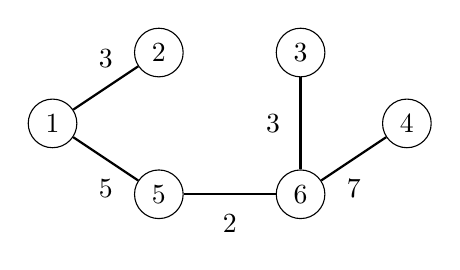
\begin{tikzpicture}[scale=0.9]
\node[draw, circle] (1) at (1.5,2) {$1$};
\node[draw, circle] (2) at (3,3) {$2$};
\node[draw, circle] (3) at (5,3) {$3$};
\node[draw, circle] (4) at (6.5,2) {$4$};
\node[draw, circle] (5) at (3,1) {$5$};
\node[draw, circle] (6) at (5,1) {$6$};

\path[draw,thick,-] (1) -- node[font=\small,label=above:3] {} (2);
%\path[draw,thick,-] (2) -- node[font=\small,label=above:5] {} (3);
%\path[draw,thick,-] (3) -- node[font=\small,label=above:9] {} (4);
\path[draw,thick,-] (1) -- node[font=\small,label=below:5] {} (5);
\path[draw,thick,-] (5) -- node[font=\small,label=below:2] {} (6);
\path[draw,thick,-] (6) -- node[font=\small,label=below:7] {} (4);
%\path[draw,thick,-] (2) -- node[font=\small,label=left:6] {} (5);
\path[draw,thick,-] (3) -- node[font=\small,label=left:3] {} (6);
\end{tikzpicture}
\end{center}
\end{samepage}

Sau đó, thuật toán sẽ không thêm bất kỳ
cạnh mới nào, vì đồ thị đã liên thông
và có một đường đi giữa hai đỉnh bất kỳ.
Đồ thị kết quả là một cây khung nhỏ nhất
với trọng số $2+3+3+5+7=20$.

\subsubsection{Tại sao thuật toán này hoạt động?}

Một câu hỏi hay là tại sao thuật toán Kruskal hoạt động.
Tại sao chiến lược tham lam lại đảm bảo rằng chúng ta
sẽ tìm thấy một cây khung nhỏ nhất?

Hãy xem điều gì xảy ra nếu cạnh có trọng số nhỏ nhất của
đồ thị \emph{không} được bao gồm trong cây khung.
Ví dụ, giả sử rằng một cây khung
cho đồ thị trước đó sẽ không chứa
cạnh có trọng số nhỏ nhất 5--6.
Chúng ta không biết cấu trúc chính xác của một cây khung như vậy,
nhưng trong mọi trường hợp, nó phải chứa một số cạnh.
Giả sử rằng cây sẽ như sau:

\begin{center}
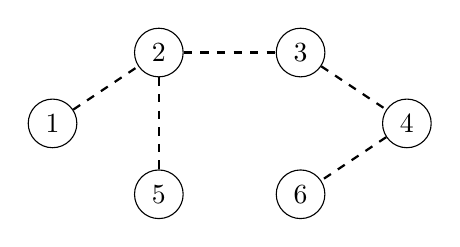
\begin{tikzpicture}[scale=0.9]
\node[draw, circle] (1) at (1.5,2) {$1$};
\node[draw, circle] (2) at (3,3) {$2$};
\node[draw, circle] (3) at (5,3) {$3$};
\node[draw, circle] (4) at (6.5,2) {$4$};
\node[draw, circle] (5) at (3,1) {$5$};
\node[draw, circle] (6) at (5,1) {$6$};

\path[draw,thick,-,dashed] (1) -- (2);
\path[draw,thick,-,dashed] (2) -- (5);
\path[draw,thick,-,dashed] (2) -- (3);
\path[draw,thick,-,dashed] (3) -- (4);
\path[draw,thick,-,dashed] (4) -- (6);
\end{tikzpicture}
\end{center}

Tuy nhiên, không thể nào cây trên
lại là một cây khung nhỏ nhất cho đồ thị.
Lý do là chúng ta có thể loại bỏ một cạnh
khỏi cây và thay thế nó bằng cạnh có trọng số nhỏ nhất 5--6.
Điều này tạo ra một cây khung có trọng số
\emph{nhỏ hơn}:

\begin{center}
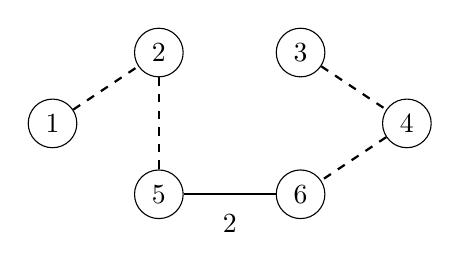
\begin{tikzpicture}[scale=0.9]
\node[draw, circle] (1) at (1.5,2) {$1$};
\node[draw, circle] (2) at (3,3) {$2$};
\node[draw, circle] (3) at (5,3) {$3$};
\node[draw, circle] (4) at (6.5,2) {$4$};
\node[draw, circle] (5) at (3,1) {$5$};
\node[draw, circle] (6) at (5,1) {$6$};

\path[draw,thick,-,dashed] (1) -- (2);
\path[draw,thick,-,dashed] (2) -- (5);
\path[draw,thick,-,dashed] (3) -- (4);
\path[draw,thick,-,dashed] (4) -- (6);
\path[draw,thick,-] (5) -- node[font=\small,label=below:2] {} (6);
\end{tikzpicture}
\end{center}

Vì lý do này, luôn tối ưu
khi bao gồm cạnh có trọng số nhỏ nhất
trong cây để tạo ra một cây khung nhỏ nhất.
Sử dụng một lập luận tương tự, chúng ta có thể chỉ ra rằng
cũng tối ưu khi thêm cạnh tiếp theo theo thứ tự trọng số
vào cây, và cứ thế.
Do đó, thuật toán Kruskal hoạt động chính xác và
luôn tạo ra một cây khung nhỏ nhất.

\subsubsection{Cài đặt}

Khi cài đặt thuật toán Kruskal,
sẽ thuận tiện khi sử dụng
biểu diễn danh sách cạnh của đồ thị.
Giai đoạn đầu tiên của thuật toán sắp xếp các
cạnh trong danh sách theo thời gian $O(m \log m)$.
Sau đó, giai đoạn thứ hai của thuật toán
xây dựng cây khung nhỏ nhất như sau:

\begin{lstlisting}
for (...) {
  if (!same(a,b)) unite(a,b);
}
\end{lstlisting}

Vòng lặp duyệt qua các cạnh trong danh sách
và luôn xử lý một cạnh $a$--$b$
trong đó $a$ và $b$ là hai đỉnh.
Cần có hai hàm:
hàm \texttt{same} xác định
liệu $a$ và $b$ có ở trong cùng một thành phần hay không,
và hàm \texttt{unite}
hợp nhất các thành phần chứa $a$ và $b$.

Vấn đề là làm thế nào để cài đặt hiệu quả
các hàm \texttt{same} và \texttt{unite}.
Một khả năng là cài đặt hàm
\texttt{same} như một phép duyệt đồ thị và kiểm tra xem
chúng ta có thể đi từ đỉnh $a$ đến đỉnh $b$ hay không.
Tuy nhiên, độ phức tạp thời gian của một hàm như vậy
sẽ là $O(n+m)$
và thuật toán kết quả sẽ chậm,
bởi vì hàm \texttt{same} sẽ được gọi cho mỗi cạnh trong đồ thị.

Chúng ta sẽ giải quyết vấn đề bằng cách sử dụng cấu trúc union-find
cài đặt cả hai hàm trong thời gian $O(\log n)$.
Do đó, độ phức tạp thời gian của thuật toán Kruskal
sẽ là $O(m \log n)$ sau khi sắp xếp danh sách cạnh.

\section{Cấu trúc Union-find}

\index{union-find structure}
\index{cấu trúc union-find}

Một \key{cấu trúc union-find} duy trì
một tập hợp các tập hợp.
Các tập hợp là rời rạc, vì vậy không có phần tử nào
thuộc về nhiều hơn một tập hợp.
Hai thao tác thời gian $O(\log n)$ được hỗ trợ:
thao tác \texttt{unite} hợp nhất hai tập hợp,
và thao tác \texttt{find} tìm đại diện
của tập hợp chứa một phần tử đã cho\footnote{Cấu trúc được trình bày ở đây
được giới thiệu vào năm 1971 bởi J. D. Hopcroft và J. D. Ullman \cite{hop71}.
Sau đó, vào năm 1975, R. E. Tarjan đã nghiên cứu một biến thể phức tạp hơn
của cấu trúc \cite{tar75} được thảo luận trong nhiều sách giáo khoa thuật toán
ngày nay.}.

\subsubsection{Cấu trúc}

Trong một cấu trúc union-find, một phần tử trong mỗi tập hợp
là đại diện của tập hợp,
và có một chuỗi từ bất kỳ phần tử nào khác của
tập hợp đến đại diện.
Ví dụ, giả sử các tập hợp là
$\{1,4,7\}$, $\{5\}$ và $\{2,3,6,8\}$:
\begin{center}
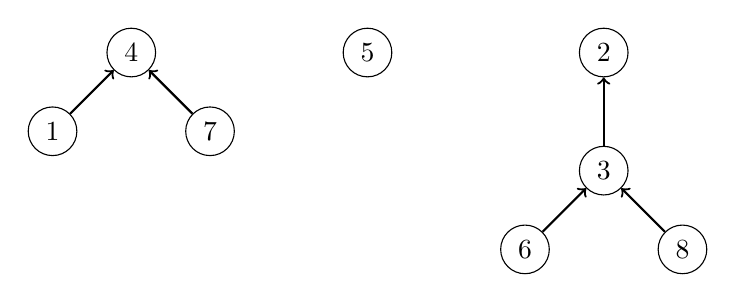
\begin{tikzpicture}
\node[draw, circle] (1) at (0,-1) {$1$};
\node[draw, circle] (2) at (7,0) {$2$};
\node[draw, circle] (3) at (7,-1.5) {$3$};
\node[draw, circle] (4) at (1,0) {$4$};
\node[draw, circle] (5) at (4,0) {$5$};
\node[draw, circle] (6) at (6,-2.5) {$6$};
\node[draw, circle] (7) at (2,-1) {$7$};
\node[draw, circle] (8) at (8,-2.5) {$8$};

\path[draw,thick,->] (1) -- (4);
\path[draw,thick,->] (7) -- (4);

\path[draw,thick,->] (3) -- (2);
\path[draw,thick,->] (6) -- (3);
\path[draw,thick,->] (8) -- (3);

\end{tikzpicture}
\end{center}
Trong trường hợp này, các đại diện
của các tập hợp là 4, 5 và 2.
Chúng ta có thể tìm đại diện của bất kỳ phần tử nào
bằng cách đi theo chuỗi bắt đầu từ phần tử đó.
Ví dụ, phần tử 2 là đại diện
cho phần tử 6, vì
chúng ta đi theo chuỗi $6 \rightarrow 3 \rightarrow 2$.
Hai phần tử thuộc cùng một tập hợp chính xác khi
đại diện của chúng giống nhau.

Hai tập hợp có thể được hợp nhất bằng cách kết nối
đại diện của một tập hợp với
đại diện của tập hợp kia.
Ví dụ, các tập hợp
$\{1,4,7\}$ và $\{2,3,6,8\}$
có thể được hợp nhất như sau:
\begin{center}
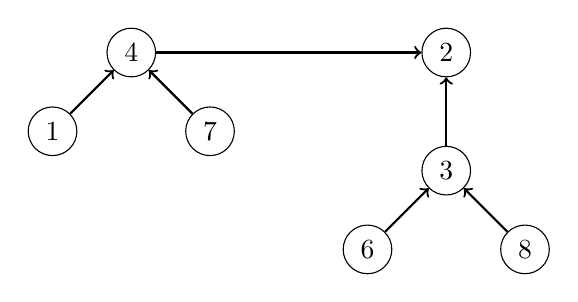
\begin{tikzpicture}
\node[draw, circle] (1) at (2,-1) {$1$};
\node[draw, circle] (2) at (7,0) {$2$};
\node[draw, circle] (3) at (7,-1.5) {$3$};
\node[draw, circle] (4) at (3,0) {$4$};
\node[draw, circle] (6) at (6,-2.5) {$6$};
\node[draw, circle] (7) at (4,-1) {$7$};
\node[draw, circle] (8) at (8,-2.5) {$8$};

\path[draw,thick,->] (1) -- (4);
\path[draw,thick,->] (7) -- (4);

\path[draw,thick,->] (3) -- (2);
\path[draw,thick,->] (6) -- (3);
\path[draw,thick,->] (8) -- (3);

\path[draw,thick,->] (4) -- (2);
\end{tikzpicture}
\end{center}

Tập hợp kết quả chứa các phần tử
$\{1,2,3,4,6,7,8\}$.
Từ đây trở đi, phần tử 2 là đại diện
cho toàn bộ tập hợp và đại diện cũ 4
trỏ đến phần tử 2.

Hiệu quả của cấu trúc union-find phụ thuộc vào
cách các tập hợp được hợp nhất.
Hóa ra chúng ta có thể tuân theo một chiến lược đơn giản:
luôn kết nối đại diện của
tập hợp \emph{nhỏ hơn} với đại diện của tập hợp \emph{lớn hơn}
(hoặc nếu các tập hợp có kích thước bằng nhau,
chúng ta có thể đưa ra một lựa chọn tùy ý).
Sử dụng chiến lược này, độ dài của bất kỳ chuỗi nào
sẽ là $O(\log n)$, vì vậy chúng ta có thể
tìm đại diện của bất kỳ phần tử nào
một cách hiệu quả bằng cách đi theo chuỗi tương ứng.

\subsubsection{Cài đặt}

Cấu trúc union-find có thể được cài đặt
bằng mảng.
Trong cài đặt sau,
mảng \texttt{link} chứa cho mỗi phần tử
phần tử tiếp theo
trong chuỗi hoặc chính phần tử đó nếu nó là
một đại diện,
và mảng \texttt{size} chỉ ra cho mỗi đại diện
kích thước của tập hợp tương ứng.

Ban đầu, mỗi phần tử thuộc về một tập hợp riêng biệt:
\begin{lstlisting}
for (int i = 1; i <= n; i++) link[i] = i;
for (int i = 1; i <= n; i++) size[i] = 1;
\end{lstlisting}

Hàm \texttt{find} trả về
đại diện cho một phần tử $x$.
Đại diện có thể được tìm thấy bằng cách đi theo
chuỗi bắt đầu tại $x$.

\begin{lstlisting}
int find(int x) {
    while (x != link[x]) x = link[x];
    return x;
}
\end{lstlisting}

Hàm \texttt{same} kiểm tra
liệu các phần tử $a$ và $b$ có thuộc cùng một tập hợp hay không.
Điều này có thể dễ dàng được thực hiện bằng cách sử dụng
hàm \texttt{find}:

\begin{lstlisting}
bool same(int a, int b) {
    return find(a) == find(b);
}
\end{lstlisting}

\begin{samepage}
Hàm \texttt{unite} hợp nhất các tập hợp
chứa các phần tử $a$ và $b$
(các phần tử phải ở trong các tập hợp khác nhau).
Hàm đầu tiên tìm các đại diện
của các tập hợp và sau đó kết nối tập hợp nhỏ hơn
với tập hợp lớn hơn.

\begin{lstlisting}
void unite(int a, int b) {
    a = find(a);
    b = find(b);
    if (size[a] < size[b]) swap(a,b);
    size[a] += size[b];
    link[b] = a;
}
\end{lstlisting}
\end{samepage}

Độ phức tạp thời gian của hàm \texttt{find}
là $O(\log n)$ giả sử rằng độ dài của mỗi
chuỗi là $O(\log n)$.
Trong trường hợp này, các hàm \texttt{same} và \texttt{unite}
cũng hoạt động trong thời gian $O(\log n)$.
Hàm \texttt{unite} đảm bảo rằng
độ dài của mỗi chuỗi là $O(\log n)$ bằng cách kết nối
tập hợp nhỏ hơn với tập hợp lớn hơn.

\section{Thuật toán Prim}

\index{Prim's algorithm}
\index{thuật toán Prim}

\key{Thuật toán Prim}\footnote{Thuật toán được
đặt theo tên của R. C. Prim, người đã công bố nó vào năm 1957 \cite{pri57}.
Tuy nhiên, thuật toán tương tự đã được phát hiện vào năm 1930
bởi V. Jarník.} là một phương pháp thay thế
để tìm một cây khung nhỏ nhất.
Thuật toán đầu tiên thêm một đỉnh tùy ý
vào cây.
Sau đó, thuật toán luôn chọn
một cạnh có trọng số nhỏ nhất
thêm một đỉnh mới vào cây.
Cuối cùng, tất cả các đỉnh đã được thêm vào cây
và một cây khung nhỏ nhất đã được tìm thấy.

Thuật toán Prim giống với thuật toán Dijkstra.
Sự khác biệt là thuật toán Dijkstra luôn
chọn một cạnh có khoảng cách từ đỉnh bắt đầu
là nhỏ nhất, nhưng thuật toán Prim chỉ đơn giản là chọn
cạnh có trọng số nhỏ nhất để thêm một đỉnh mới vào cây.

\subsubsection{Ví dụ}

Hãy xem xét cách thuật toán Prim hoạt động
trong đồ thị sau:

\begin{center}
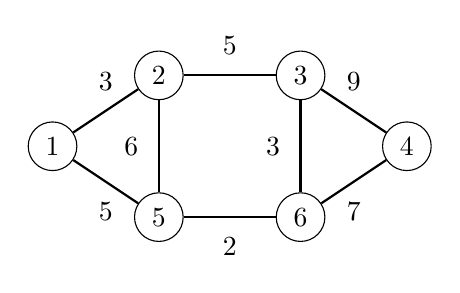
\begin{tikzpicture}[scale=0.9]
\node[draw, circle] (1) at (1.5,2) {$1$};
\node[draw, circle] (2) at (3,3) {$2$};
\node[draw, circle] (3) at (5,3) {$3$};
\node[draw, circle] (4) at (6.5,2) {$4$};
\node[draw, circle] (5) at (3,1) {$5$};
\node[draw, circle] (6) at (5,1) {$6$};
\path[draw,thick,-] (1) -- node[font=\small,label=above:3] {} (2);
\path[draw,thick,-] (2) -- node[font=\small,label=above:5] {} (3);
\path[draw,thick,-] (3) -- node[font=\small,label=above:9] {} (4);
\path[draw,thick,-] (1) -- node[font=\small,label=below:5] {} (5);
\path[draw,thick,-] (5) -- node[font=\small,label=below:2] {} (6);
\path[draw,thick,-] (6) -- node[font=\small,label=below:7] {} (4);
\path[draw,thick,-] (2) -- node[font=\small,label=left:6] {} (5);
\path[draw,thick,-] (3) -- node[font=\small,label=left:3] {} (6);

%\path[draw=red,thick,-,line width=2pt] (5) -- (6);
\end{tikzpicture}
\end{center}
Ban đầu, không có cạnh nào giữa các đỉnh:
\begin{center}
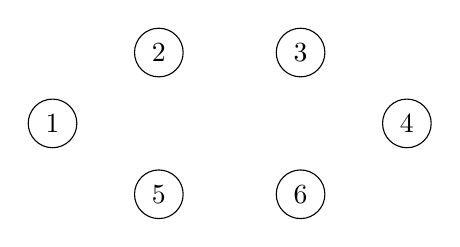
\begin{tikzpicture}[scale=0.9]
\node[draw, circle] (1) at (1.5,2) {$1$};
\node[draw, circle] (2) at (3,3) {$2$};
\node[draw, circle] (3) at (5,3) {$3$};
\node[draw, circle] (4) at (6.5,2) {$4$};
\node[draw, circle] (5) at (3,1) {$5$};
\node[draw, circle] (6) at (5,1) {$6$};
%\path[draw,thick,-] (1) -- node[font=\small,label=above:3] {} (2);
%\path[draw,thick,-] (2) -- node[font=\small,label=above:5] {} (3);
%\path[draw,thick,-] (3) -- node[font=\small,label=above:9] {} (4);
%\path[draw,thick,-] (1) -- node[font=\small,label=below:5] {} (5);
%\path[draw,thick,-] (5) -- node[font=\small,label=below:2] {} (6);
%\path[draw,thick,-] (6) -- node[font=\small,label=below:7] {} (4);
%\path[draw,thick,-] (2) -- node[font=\small,label=left:6] {} (5);
%\path[draw,thick,-] (3) -- node[font=\small,label=left:3] {} (6);
\end{tikzpicture}
\end{center}
Một đỉnh tùy ý có thể là đỉnh bắt đầu,
vì vậy hãy chọn đỉnh 1.
Đầu tiên, chúng ta thêm đỉnh 2 được nối bằng
một cạnh có trọng số 3:
\begin{center}
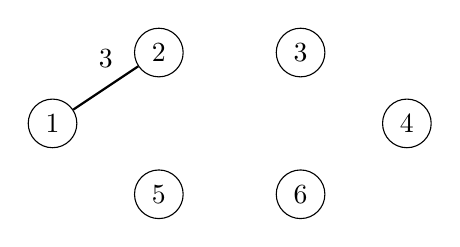
\begin{tikzpicture}[scale=0.9]
\node[draw, circle] (1) at (1.5,2) {$1$};
\node[draw, circle] (2) at (3,3) {$2$};
\node[draw, circle] (3) at (5,3) {$3$};
\node[draw, circle] (4) at (6.5,2) {$4$};
\node[draw, circle] (5) at (3,1) {$5$};
\node[draw, circle] (6) at (5,1) {$6$};
\path[draw,thick,-] (1) -- node[font=\small,label=above:3] {} (2);
%\path[draw,thick,-] (2) -- node[font=\small,label=above:5] {} (3);
%\path[draw,thick,-] (3) -- node[font=\small,label=above:9] {} (4);
%\path[draw,thick,-] (1) -- node[font=\small,label=below:5] {} (5);
%\path[draw,thick,-] (5) -- node[font=\small,label=below:2] {} (6);
%\path[draw,thick,-] (6) -- node[font=\small,label=below:7] {} (4);
%\path[draw,thick,-] (2) -- node[font=\small,label=left:6] {} (5);
%\path[draw,thick,-] (3) -- node[font=\small,label=left:3] {} (6);
\end{tikzpicture}
\end{center}

Sau đó, có hai cạnh có trọng số 5,
vì vậy chúng ta có thể thêm đỉnh 3 hoặc đỉnh 5 vào cây.
Hãy thêm đỉnh 3 trước:
\begin{center}
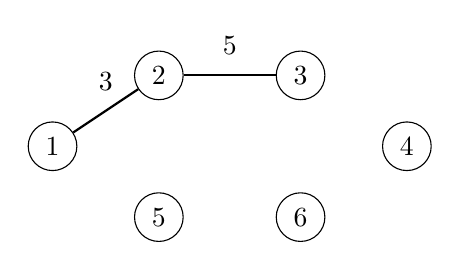
\begin{tikzpicture}[scale=0.9]
\node[draw, circle] (1) at (1.5,2) {$1$};
\node[draw, circle] (2) at (3,3) {$2$};
\node[draw, circle] (3) at (5,3) {$3$};
\node[draw, circle] (4) at (6.5,2) {$4$};
\node[draw, circle] (5) at (3,1) {$5$};
\node[draw, circle] (6) at (5,1) {$6$};
\path[draw,thick,-] (1) -- node[font=\small,label=above:3] {} (2);
\path[draw,thick,-] (2) -- node[font=\small,label=above:5] {} (3);
%\path[draw,thick,-] (3) -- node[font=\small,label=above:9] {} (4);
%\path[draw,thick,-] (1) -- node[font=\small,label=below:5] {} (5);
%\path[draw,thick,-] (5) -- node[font=\small,label=below:2] {} (6);
%\path[draw,thick,-] (6) -- node[font=\small,label=below:7] {} (4);
%\path[draw,thick,-] (2) -- node[font=\small,label=left:6] {} (5);
%\path[draw,thick,-] (3) -- node[font=\small,label=left:3] {} (6);
\end{tikzpicture}
\end{center}

\begin{samepage}
Quá trình tiếp tục cho đến khi tất cả các đỉnh đã được đưa vào cây:
\begin{center}
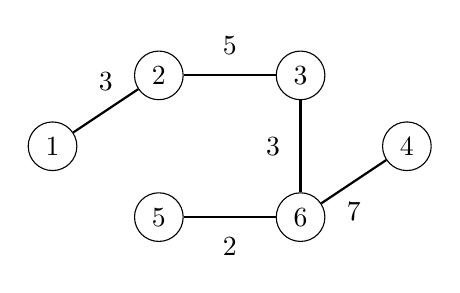
\begin{tikzpicture}[scale=0.9]
\node[draw, circle] (1) at (1.5,2) {$1$};
\node[draw, circle] (2) at (3,3) {$2$};
\node[draw, circle] (3) at (5,3) {$3$};
\node[draw, circle] (4) at (6.5,2) {$4$};
\node[draw, circle] (5) at (3,1) {$5$};
\node[draw, circle] (6) at (5,1) {$6$};
\path[draw,thick,-] (1) -- node[font=\small,label=above:3] {} (2);
\path[draw,thick,-] (2) -- node[font=\small,label=above:5] {} (3);
%\path[draw,thick,-] (3) -- node[font=\small,label=above:9] {} (4);
%\path[draw,thick,-] (1) -- node[font=\small,label=below:5] {} (5);
\path[draw,thick,-] (5) -- node[font=\small,label=below:2] {} (6);
\path[draw,thick,-] (6) -- node[font=\small,label=below:7] {} (4);
%\path[draw,thick,-] (2) -- node[font=\small,label=left:6] {} (5);
\path[draw,thick,-] (3) -- node[font=\small,label=left:3] {} (6);
\end{tikzpicture}
\end{center}
\end{samepage}

\subsubsection{Cài đặt}

Giống như thuật toán Dijkstra, thuật toán Prim có thể được
cài đặt hiệu quả bằng hàng đợi ưu tiên.
Hàng đợi ưu tiên nên chứa tất cả các đỉnh
có thể được kết nối với thành phần hiện tại bằng
một cạnh duy nhất, theo thứ tự tăng dần của trọng số
của các cạnh tương ứng.

Độ phức tạp thời gian của thuật toán Prim là
$O(n + m \log m)$ bằng với độ phức tạp thời gian
của thuật toán Dijkstra.
Trong thực tế, thuật toán Prim và Kruskal
đều hiệu quả, và việc lựa chọn thuật toán
là vấn đề sở thích.
Tuy nhiên, hầu hết các lập trình viên thi đấu đều sử dụng thuật toán Kruskal.